\section{Hausdorff distance}
\label{hausdorff_distance_chapter}
\nblink{brats/15a\_hausdorff\_distance.ipynb}

In the previous section, we showed differences between the reference neural network output and the output of images where a part of them has been masked by a circle.
Showing this difference for all the applied masks is impractical, a single visualization which shows all the output segment changes would be helpful.
A first step is getting a single number for the difference of the two segments (unchanged reference segment, output segment from masked image).

A way to calculate the similarity (or difference) between two matrices (the output segments of the neural network are 2D matrices) is a distance function.

We choose the Hausdorff distance function because it has a specific property that is helpful for our requirements: A slightly moved object is still considered more similar to
an object with a completely different shape, even when the changed pixel count is exactly the same.

% The formula for the Hausdorff distance is:
% $ _{\mathrm {H} }(X,Y)=\max\{\,\sup _{x\in X}\inf _{y\in Y}d(x,y),\,\sup _{y\in Y}\inf _{x\in X}d(x,y)\} $
% $X$ and $Y$ are the two sets/matrices which are compared. $d(x,y)$ is the distance between two points. $inf$ and $sup$ are the Infimum and supremum: When comparing two
% ordered sets A and B, the infinum of A in comparison to B is the biggest item in A that is still smaller than all items of B. The inverse is the supremum,
% the smallest item in A that is still bigger 
% \begin{figure}[H]
% \centering
% 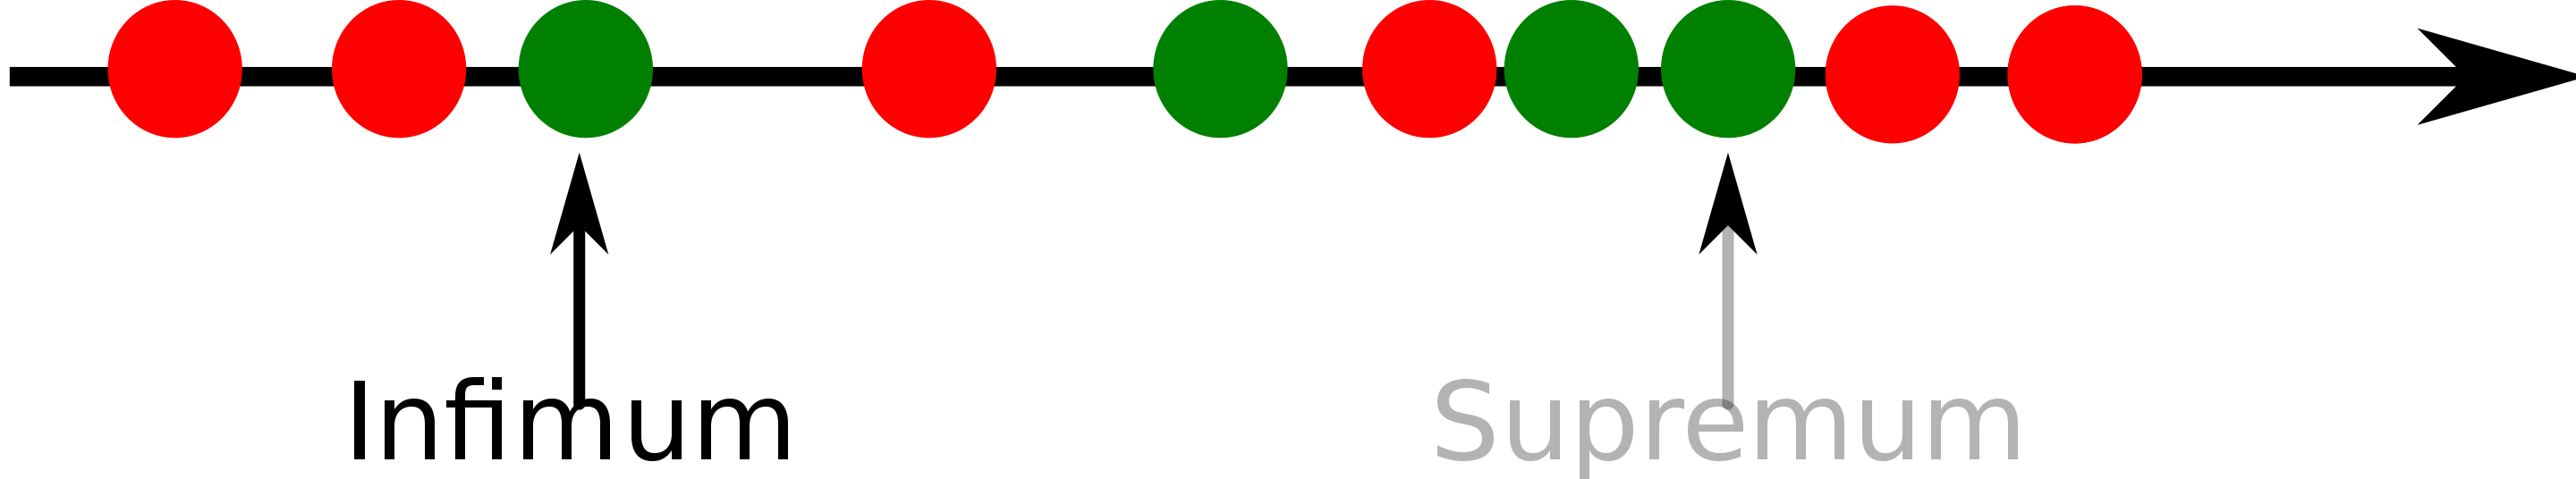
\includegraphics[width=8cm]{chapters/06_hdm/images/inf_sup.png}
% \caption{Visualization of the Infimum and supremum \cite{hausdorffdistanceimage2}}
% \label{inf_sup}
% \end{figure}

Intuitively, the Hausdorff distance searches the two maximal distances between sets (A to B and B to a) and returns the higher one as the distance.
The maximal distance from set A to set B is the biggest distance between a pixel from set A to a pixel in set B, but the distance from the pixel from set A to the pixel B has to be the smallest distance from pixel A to any pixel on the set B.

A visual explanation of the Hausdorff distance is given in Figure \ref{hausdorff_distance}.

\begin{figure}[H]
\centering
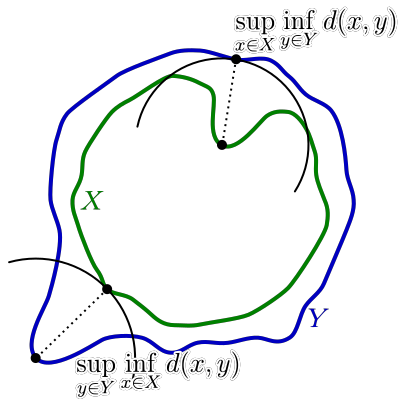
\includegraphics[width=6cm]{chapters/06_hdm/images/hausdorff_distance.png}
\caption{Visualization of the Hausdorff distance. The Hausdorff distance from set Y to set X is the maximal distance of a point in set Y to a point in set X, but this distance still has to be the smallest distance from the point on set Y to any point on set X.\cite{hausdorffdistanceimage}}
\label{hausdorff_distance}
\end{figure}

A naive implementation of the algorithm in Python is given in Listing \ref{hausdorff_distance_python}.

\begin{listing}[H]
\begin{minted}{python}
def inner_hausdorff(X, Y):
    minimal_distances = []
    for x in X:
        distances = []
        for y in Y:
            distances.append(distance(x,y))
        min_distance = min(distances)  # infinum
        minimal_distances.append(min_distance)
    return max(minimal_distances) # supremum

def hausdorff_distance(X, Y):
    return max(inner_hausdorff(X, Y), inner_hausdorff(Y, X))
\end{minted}
\caption{Naive implementation of the Hausdorff distance in Python}
\label{hausdorff_distance_python}
\end{listing}

\subsection{Examples}
The following visualizations show samples of shapes compared with the Hausdorff distance function.

\begin{figure}[H]
    \centering
    \begin{subfigure}{.35\textwidth}
        \centering
        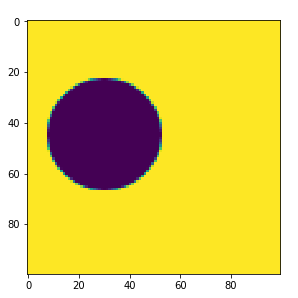
\includegraphics[width=\linewidth]{chapters/06_hdm/images/hdm_original.png}
        \caption{Original shape}
    \end{subfigure}%
    \begin{subfigure}{.35\textwidth}
        \centering
        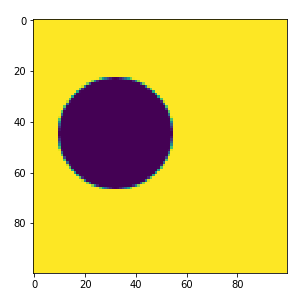
\includegraphics[width=\linewidth]{chapters/06_hdm/images/hdm_moved1.png}
        \caption{Shape moved slightly to the right}
    \end{subfigure}
    \caption{Hausdorff distance between the left and the right figure: 476.}
    \label{hdm_moved1}
\end{figure}

Figure \ref{hdm_moved1} shows a slightly moved circle, the Hausdorff distance between the images is quite low with 476.

\begin{figure}[H]
    \centering
    \begin{subfigure}{.35\textwidth}
        \centering
        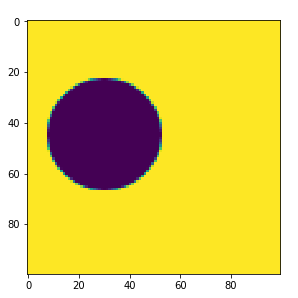
\includegraphics[width=\linewidth]{chapters/06_hdm/images/hdm_original.png}
        \caption{Original shape}
    \end{subfigure}%
    \begin{subfigure}{.35\textwidth}
        \centering
        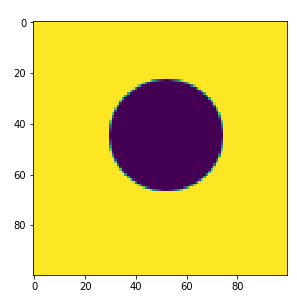
\includegraphics[width=\linewidth]{chapters/06_hdm/images/hdm_moved2.png}
        \caption{Shape moved to the right}
    \end{subfigure}
    \caption{Hausdorff distance between the left and the right figure: 1656. }
    \label{hdm_moved2}
\end{figure}

Figure \ref{hdm_moved2} shows a shape that is moved to right, showing a bigger Hausdorff distance than in Figure \ref{hdm_moved1} with 1565.

\begin{figure}[H]
    \centering
    \begin{subfigure}{.35\textwidth}
        \centering
        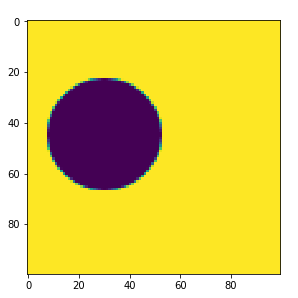
\includegraphics[width=\linewidth]{chapters/06_hdm/images/hdm_original.png}
        \caption{Original shape}
    \end{subfigure}%
    \begin{subfigure}{.35\textwidth}
        \centering
        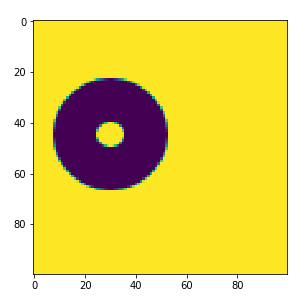
\includegraphics[width=\linewidth]{chapters/06_hdm/images/hdm_hole.png}
        \caption{Shape moved to the right}
    \end{subfigure}
    \caption{Hausdorff distance between the left and the right figure: 840. }
    \label{hdm_hole}
\end{figure}

Figure \ref{hdm_hole} shows the shape at the same position but with a hole in the middle.

\begin{figure}[H]
    \centering
    \begin{subfigure}{.35\textwidth}
        \centering
        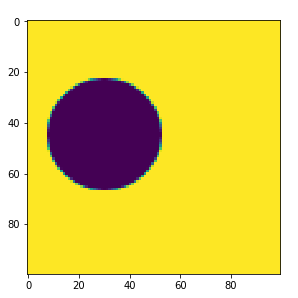
\includegraphics[width=\linewidth]{chapters/06_hdm/images/hdm_original.png}
        \caption{Original shape}
    \end{subfigure}%
    \begin{subfigure}{.35\textwidth}
        \centering
        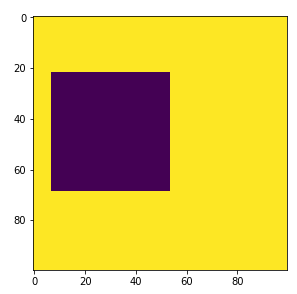
\includegraphics[width=\linewidth]{chapters/06_hdm/images/hdm_square.png}
        \caption{Shape moved to the right}
    \end{subfigure}
    \caption{Hausdorff distance between the left and the right figure: 1197. }
    \label{hdm_square}
\end{figure}

Figure \ref{hdm_square} shows the shape transformed into a square. The distance between the shapes is much bigger compared the the shape with a hole in it in Figure \ref{hdm_hole}, even when the
changed count of pixels is similar.


\begin{figure}[H]
    \centering
    \begin{subfigure}{.35\textwidth}
        \centering
        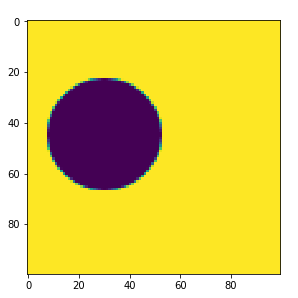
\includegraphics[width=\linewidth]{chapters/06_hdm/images/hdm_original.png}
        \caption{Original shape}
    \end{subfigure}%
    \begin{subfigure}{.35\textwidth}
        \centering
        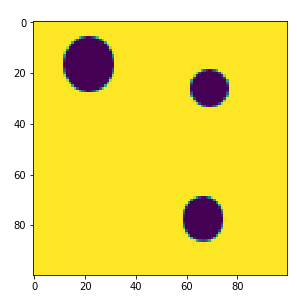
\includegraphics[width=\linewidth]{chapters/06_hdm/images/hdm_smaller_circles.png}
        \caption{Shape moved to the right}
    \end{subfigure}
    \caption{Hausdorff distance between the left and the right figure: 1353.}
    \label{hdm_smaller_circles}
\end{figure}

Figure \ref{hdm_smaller_circles} shows the shape completely replaced by three smaller circles. The Hausdorff distance is the highest of all the sample images with 1353.
